\documentclass[11pt]{article}
\usepackage[margin=1in]{geometry}
\usepackage{booktabs,graphicx,amsmath}
\title{Online Q-learning on the same gradual scorecard race}
\author{}
\date{}
\begin{document}
\maketitle

\section{What can differ from UCB}

The arms, the batch of 200, and the pseudo-outcome share are the relocation MVP.
The reward is still negative batch mean squared error. In a stateless bandit,
Sarsa and Q-learning select the same arm, and a step size \(1/n\) is the sample
mean already inside UCB. The updates below are the ones that can actually move
the index: a constant step, two tables, a speedy extrapolation, a softmax, and
a window of the last eight rewards. Constant-step Q, double Q, the bonus,
and the window are also run with the FSDS tax at \(\eta=2\). Speedy Q and
Boltzmann are reported without that tax. The first four rounds still pull each
arm once. A table is
initialized at the first reward of that arm. A zero start would be optimistic,
because the rewards are negative.

Constant \(\alpha\) forgets. Greedy Q never refreshes an arm it has stopped
pulling, so a value frozen before the ramp cannot follow the fresh block.
A bonus, a softmax, or a sliding window is what lets the other arms move.
The tax is subtracted from every arm's index, not only from the arm just pulled.

\section{Relocation stays with the tax}

UCB at \(\eta=2\) remains the reference. Its median post-shift excess is
17.6, against 34.6
for plain UCB and 24.6 for discounted UCB.
Greedy Q at \(\alpha=0.2\) is 28.8. That gap
against UCB at \(\eta=2\) clears the larger seed standard deviation on
6/6 pools. The same tax on the frozen
value gives 18.5. Q plus a UCB bonus, without
the tax, is 25.5, next to discounted UCB, and
it clears discounted UCB on 1/6 pools.
The bonus with the tax is 17.8. Speedy Q is
the lowest untaxed rule at 21.9, and UCB at
\(\eta=2\) still clears it on 5/6 pools.
Double Q updates one table at random and finishes at
40.5. Boltzmann pays during the stationary window
(early excess 38.6, against
16.6 for UCB) and finishes at
62.6.

On covertype, Gaussian-30, and Student-$t_5$, all four seeds of Q-plus-bonus at \(\eta=2\) match
UCB at \(\eta=2\). The match is 15 of 24 seed-pool pairs, and the
eight-step window with the same bonus and tax matches on 15 of 24
(covertype, Gaussian-30, and Student-$t_5$). Once the share is sharp, the tax is choosing the arm.
The taxed bonus rule undercuts UCB at \(\eta=2\) by more than the seed standard
deviation on California (0.7, sd 0.7, against 1.5, sd 0.6). The absolute gap is under one excess MSE, and the
median across pools stays with UCB at \(\eta=2\)
(17.6 against
17.8).

\section{The sign flip is the one Q gain}

On a gradual sign flip the tax is the wrong instrument. UCB sits at
166.1 and UCB at \(\eta=2\) at
187.4. Discounted UCB is
99.2. Q plus a UCB bonus, with the tax off, is
74.0. That gap clears the larger seed standard
deviation against discounted UCB on 5/6
pools and against plain UCB on 6/6.
The pool that stays inside the seed noise is California, where the bonus rule is 20.3 (sd 3.0) and discounted UCB is 22.4 (sd 1.0). Speedy Q is
79.4 and clears discounted UCB on
3/6 pools, so the median alone overstates it.
The post-shift hit rate of Q plus the bonus is 0.22.
The rule still misses the live card on most batches after the ramp. This is a
side result. It does not replace the relocation index.

\section{Noise growth}

When the best card never changes, forgetting a still-valid history costs excess.
Thompson sampling is 1.1 and clears UCB on
6/6 pools. UCB is
4.0 and UCB at \(\eta=2\) is
3.7. Greedy Q at \(\alpha=0.05\) is
6.1, speedy Q is
5.2, and Q plus a bonus is
15.2. UCB at \(\eta=2\) clears that bonus rule
on 6/6 pools.

The relocation index stays UCB minus \(\eta\sigma w_k\) at \(\eta=2\).
The sign-flip gain of Q plus a bonus is a side record, and on that ramp the tax
stays off.

\begin{table}[ht]
\centering
\caption{Median, across six pools, of the four-seed mean post-shift excess.}
\resizebox{\textwidth}{!}{%
\begin{tabular}{lcccccccccccc}
\toprule
scenario & UCB & DUCB & UCB-H2 & TS & QL20 & QL20-H2 & QL-UCB & QL-UCB-H2 & DQL & SQL & BOLT & QWIN-UCB-H2 \\
\midrule
gradual\_relocate & 34.6 & 24.6 & 17.6 & 87.0 & 28.8 & 18.5 & 25.5 & 17.8 & 40.5 & 21.9 & 62.6 & 17.8 \\
gradual\_flip & 166.1 & 99.2 & 187.4 & 214.5 & 103.4 & 165.2 & 74.0 & 160.2 & 138.0 & 79.4 & 133.7 & 162.5 \\
gradual\_noise & 4.0 & 7.3 & 3.7 & 1.1 & 8.1 & 7.7 & 15.2 & 12.2 & 8.7 & 5.2 & 38.7 & 12.1 \\
\bottomrule
\end{tabular}}
\end{table}

\begin{table}[ht]
\centering
\caption{Gradual relocation. Mean post-shift excess over four seeds, seed standard deviation in parentheses.}
\resizebox{\textwidth}{!}{%
\begin{tabular}{lcccccc}
\toprule
pool & UCB & UCB-H2 & QL20 & QL-UCB & QL-UCB-H2 & QWIN-UCB-H2 \\
\midrule
AR(1) & 18.2 (1.6) & 8.8 (0.5) & 13.3 (1.7) & 14.4 (0.3) & 9.9 (1.9) & 10.3 (1.6) \\
California & 4.2 (0.6) & 1.5 (0.6) & 4.4 (1.2) & 1.0 (0.7) & 0.7 (0.7) & 0.7 (0.3) \\
covertype & 73.1 (20.7) & 31.2 (1.2) & 49.6 (16.8) & 41.9 (0.9) & 31.2 (1.2) & 31.2 (1.2) \\
Gaussian-12 & 22.9 (0.4) & 10.3 (0.1) & 19.0 (3.9) & 18.8 (0.5) & 10.6 (0.5) & 10.6 (0.5) \\
Gaussian-30 & 50.6 (8.5) & 25.1 (1.5) & 44.8 (3.5) & 33.2 (1.3) & 25.1 (1.5) & 25.1 (1.5) \\
Student-$t_5$ & 46.3 (4.7) & 25.0 (1.1) & 38.6 (6.3) & 32.3 (1.1) & 25.0 (1.1) & 25.0 (1.1) \\
\bottomrule
\end{tabular}}
\end{table}

\begin{table}[ht]
\centering
\caption{Gradual sign flip. Mean post-shift excess over four seeds, seed standard deviation in parentheses.}
\resizebox{\textwidth}{!}{%
\begin{tabular}{lccccc}
\toprule
pool & UCB & DUCB & UCB-H2 & QL-UCB & SQL \\
\midrule
AR(1) & 39.9 (6.4) & 34.9 (1.3) & 66.8 (1.8) & 26.8 (0.8) & 34.6 (4.0) \\
California & 28.0 (2.9) & 22.4 (1.0) & 46.4 (2.0) & 20.3 (3.0) & 24.0 (4.2) \\
covertype & 349.6 (7.2) & 202.9 (17.8) & 364.2 (16.6) & 158.3 (21.4) & 153.3 (22.7) \\
Gaussian-12 & 63.5 (10.5) & 49.8 (7.2) & 104.3 (6.8) & 40.1 (2.8) & 50.1 (7.1) \\
Gaussian-30 & 272.3 (14.8) & 148.7 (15.7) & 281.9 (19.0) & 107.8 (9.1) & 108.6 (4.5) \\
Student-$t_5$ & 268.7 (20.5) & 155.8 (18.2) & 270.4 (15.7) & 112.2 (13.2) & 115.3 (5.6) \\
\bottomrule
\end{tabular}}
\end{table}


\begin{figure}[ht]
\centering
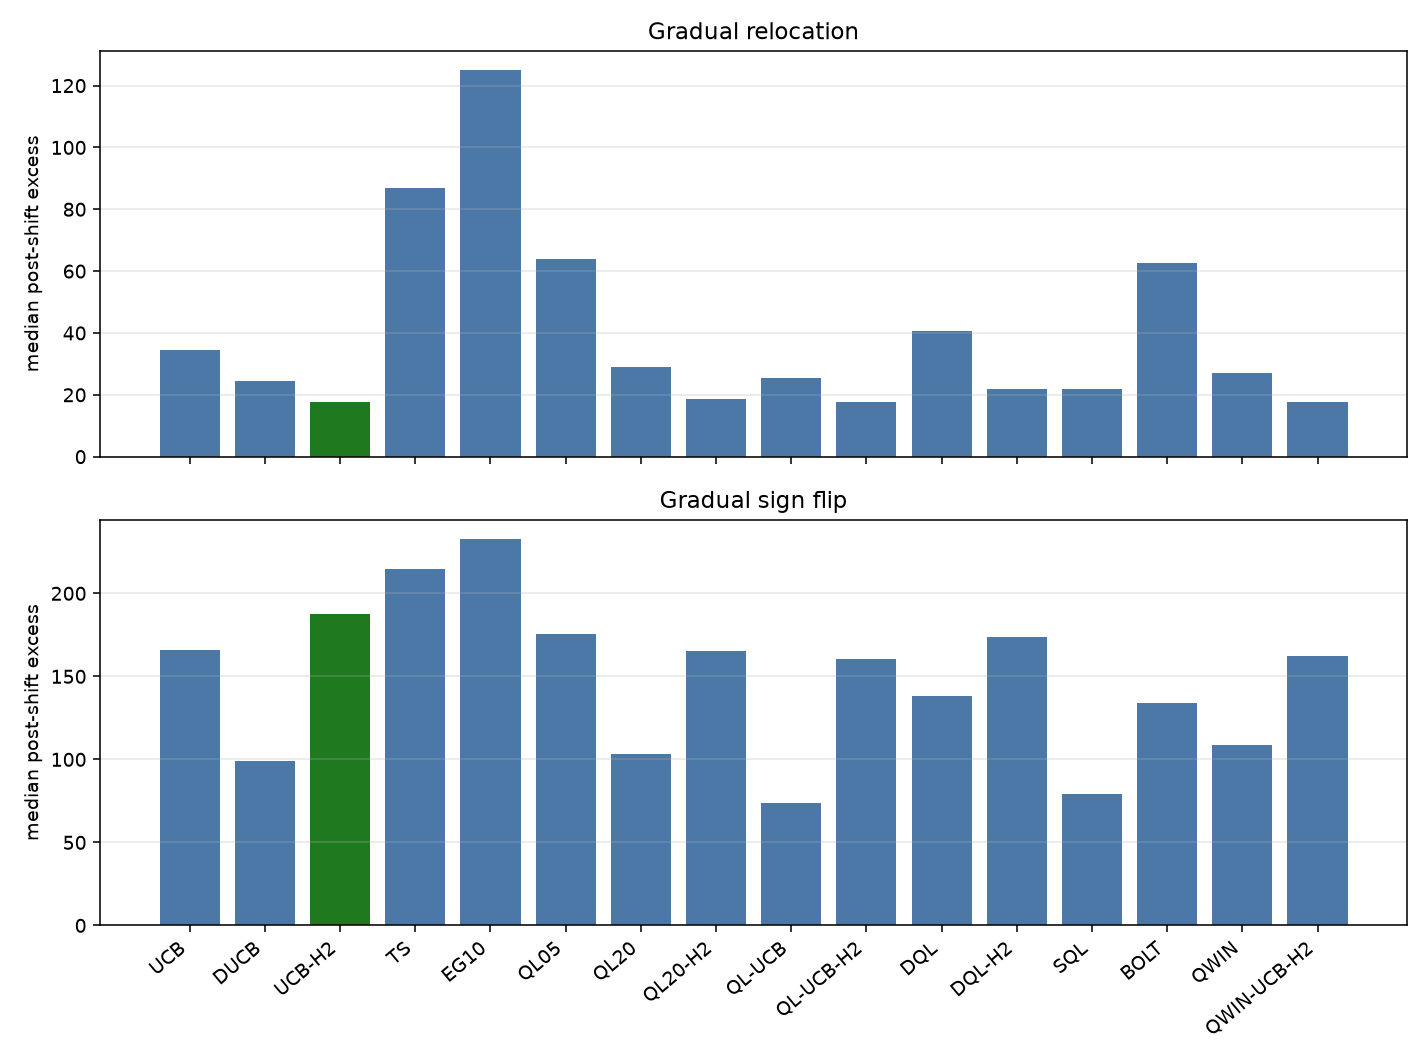
\includegraphics[width=\textwidth]{ql_bars.png}
\caption{Median post-shift excess across the six pools.
UCB at \(\eta=2\) is marked in green. The top panel is gradual relocation.
The bottom panel is the gradual sign flip, where that tax raises the excess.}
\end{figure}
\end{document}
